\documentclass[border=2pt]{standalone}
\usepackage{amsmath}
\usepackage{tikz}
\usetikzlibrary{intersections}
\usetikzlibrary{arrows}
\usetikzlibrary{quotes,angles}
\usepackage{amsmath}
\usepackage{xcolor}

\begin{document}

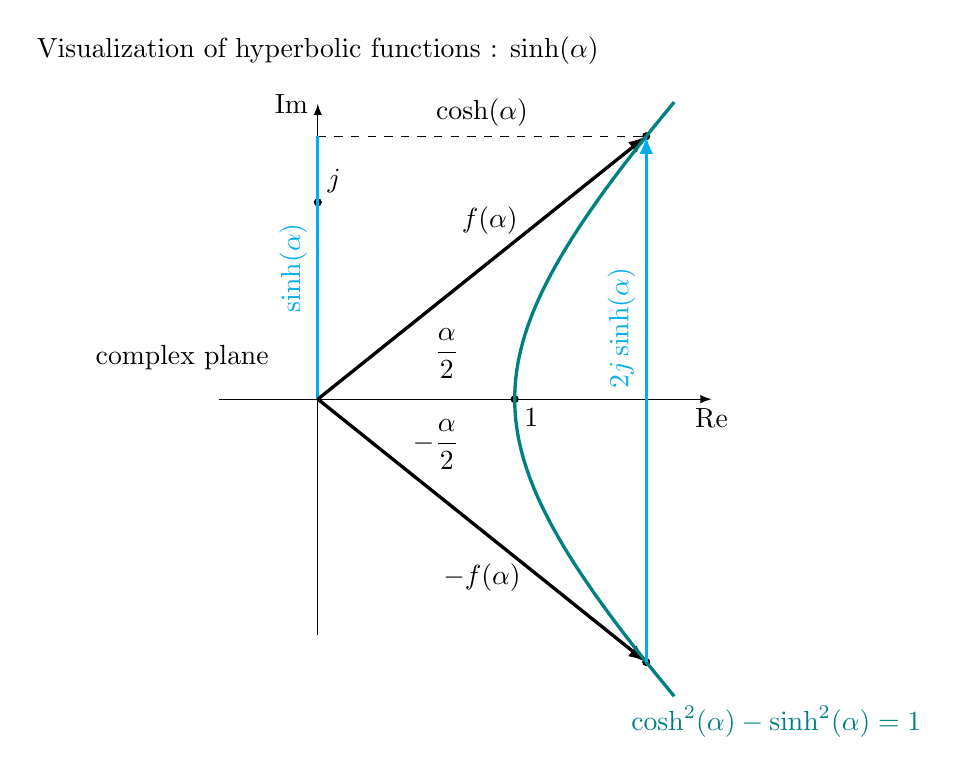
\begin{tikzpicture}[scale=2.5]

% Draw x and y axis lines
\draw [->,>=latex] (-0.5,0) -- (2.00,0) node [below] {$\mathrm{Re}$};
\draw [->,>=latex] (0,-1.2) -- (0,1.50) node [left ] {$\mathrm{Im}$};
\node[above left] at (-0.2, 0.1) {complex plane};
\filldraw[black] (1,0) circle (0.5pt) node[below right] {$1$} ;
\filldraw[black] (0,1) circle (0.5pt) node[above right] {$j$} ;
\node[above] at (0.0,1.65) {Visualization of hyperbolic functions : $\sinh(\alpha)$};

% Draw a circle at the origin of radius 1
%\draw (0,0) circle (1);

%\draw [very thin, dashed] (-1.5,-1.5) -- ( 1.5, 1.5) node[above] {$y=x$} ;
%\draw [very thin, dashed] (-1.5, 1.5) -- ( 1.5,-1.5) ;

\pgfmathsetmacro{\angle}{1.1}
\pgfmathsetmacro{\length}{\angle}

\filldraw[black] ({ cosh(\angle)}, { sinh(\angle)}) circle (0.5pt) ;
\filldraw[black] ({ cosh(\angle)}, {-sinh(\angle)}) circle (0.5pt) ;

\draw [very thin, dashed] ( 0.0, { sinh(\angle)}) -- node[above] {$\cosh(\alpha)$}  ({ cosh(\angle)}, { sinh(\angle)}) ;
\draw [very thick, cyan] ( 0.0, 0.0) -- node[above, rotate=90] {$\sinh(\alpha)$}  ( 0.0, { sinh(\angle)}) ;

\draw[very thick, ->,>=latex] (0,0) -- node[above=8pt] {$\;\;f(\alpha)$} ({ cosh(\angle)}, { sinh(\angle)}) ;
\draw[very thick, ->,>=latex] (0,0) -- node[below=8pt] {$-f(\alpha)$} ({ cosh(\angle)}, {-sinh(\angle)}) ;



% 画双曲线
\draw[very thick,smooth,variable=\x, teal] plot[domain=-\angle-0.1:\angle+0.1] ({ cosh(\x)}, {sinh(\x)}) ;
\node[below right, teal] at ({ cosh(\angle-0.1)}, {-sinh(\angle+0.1)}) {$\cosh^2(\alpha) - \sinh^2(\alpha) = 1$} ;
%\draw[very thick,smooth,variable=\x, teal] plot[domain=-1.2:1.2] ({-cosh(\x)}, {sinh(\x)}) ;

\draw[very thick, ->,>=latex, cyan] ({ cosh(\angle)}, {-sinh(\angle)}) -- node[above right, rotate=90] {$2j\sinh(\alpha)$} ({ cosh(\angle)}, { sinh(\angle)}) ;

\node[above=4pt ] at (0.6, 0) {$\;\;\:\dfrac{\alpha}{2}$} ;
\node[below=4pt ] at (0.6, 0) {$ -\dfrac{\alpha}{2}$} ;

\end{tikzpicture}

\end{document}
